\chapter{TrackCIS, un outil au service de l'interopérabilité des applications
hospitalières}
	\paragraph{}
	Cette première grande partie est une introduction du projet sur lequel porte ce
	mémoire. Ce projet s'inscrit dans des enjeux propres à la société Xperis et
	porte sur l'outil TrackCIS, console de supervision de l'EAI Cloverleaf. Nous
	nous attacherons donc ici à présenterles différents éléments importants de
	notre étude de façon à en cerner tous les enjeux et à mettre en place une
	méthodologie adapté.

	\subsection{TrackCIS est une console de supervision de l'EAI Cloverleaf}
		\paragraph{}
		Commençons par définir quelques notions techniques qui nous seront utiles,
		sinon indispensables pour la suite : les EAI et leurs consoles de supervision.
		
		\subsubsection{Qu'est-ce qu'un EAI ?}
			\paragraph{}% Interopérabilité
			EAI signifie Intégration d'Application d'Entreprise. Pour bien comprendre de
			quoi il s'agit et quel rôle tient un tel outil dans un SI, il nous faut
			comprendre la notion d'interopérabilité. Il est important
			de préciser que nous ne parlerons dans cette partie - et plus généralement
			tout au long de ce document - que des EAI dans le monde hospitalier. En
			effet, de nombreuses entreprises ou organismes de tous les secteurs utilisent
			de tels outils. Dans notre cas nous nous focaliserons uniquement sur les EAI du
			monde hospitalier et nous chercherons à comprendre ce que sont les EAI au
			travers d'exemples de ce secteur.\newline
			Selon la définition du dictionnaire Larousse, l'interopérabilité est la
			"capacité de matériels, de logiciels ou de protocoles différents à
			fonctionner ensemble et à partager des informations"
			\citep{larousse_definitions_interop}. Si l'on transpose cette définition au
			monde de l'hôpital, l'interopérabilité correspond à la capacité des
			différents logiciels (ou applicatifs) métier à fonctionner ensemble. Il
			existe une grande diversité d'applicatifs métier dans ce secteur. Le
			\ref{tableau 1} offre un aperçu de quelques fonctions
			remplies par les logiciels que l'on peut trouver dans un hôpital.
			\begin{table}[!h]
				\centering
				\begin{tabular}{| p{4cm} | p{10cm} |} %Exemples des principaux logiciels
				% métier
					\hline
					\thead{Type de fonctionnalité}&\thead{Description}
					\\
					\hline
					La GAM (Gestion Administrative des Malades)
					&
					Bla bla bla bla
					\\
					\hline
					Le DPI (Dossier Patient Informatisé)
					&
					Le DPI 
					DPI et GAM sont les deux princpaux outils utilisés dans les centres
					hospitéliers. De nombreux éditeurs proposent des logiciels permettant de
					remplir ces fonctions.\\
					\hline
				\end{tabular}
				\caption{\label{tableau 1}Quelques fonctions assurées par les
				logiciels métier présents dans les hôpitaux \citep{interopsante_guide_2015}.}
			\end{table}
			Or ces différents outils ont bien souvent été développés par des sociétés
			différentes. En outre, ces outils sont spécialisés dans quelques fonctions
			bien précises : comptabilité, enregistrement des patients, gestion des
			stocks de pharmacie\ldots Dans la plupart des cas, leur conception ne leur
			permet pas de fonctionner ensemble, ce qui pourtant peut s'avérer utile. Par
			exemple, le logiciel gérant les stocks de la pharmacie peut avoir besoin
			d'informations sur les prescriptions faites par les médecins aux patients. De
			même, les données sur les patients saisies à l'arrivée de ces derniers
			peuvent intéresser les médecins dans le logiciel gérant les dossiers
			patients.
			En résumé, il est nécessaire pour ces différentes applications de partager
			des données.
			
			\paragraph{}% L'EAI est la solution au problème de l'interopérabilité
			C'est ici qu'entre en jeux l'EAI. Il s'agit d'un outil qui établit des
			connexions entre les applications métier. Il va par exemple collecter
			certaines données émises par le logiciel de gestion des entrées patients
			pour les injecter dans l'outil de gestion des dossiers patients. Plus
			généralement, il transfert des données émises par un outil A pour les
			mettre à disposition d'un outil B \ref{Figure 1}.\newline
			
			% Schéma général d'un EAI
			\begin{figure}
				\centering
				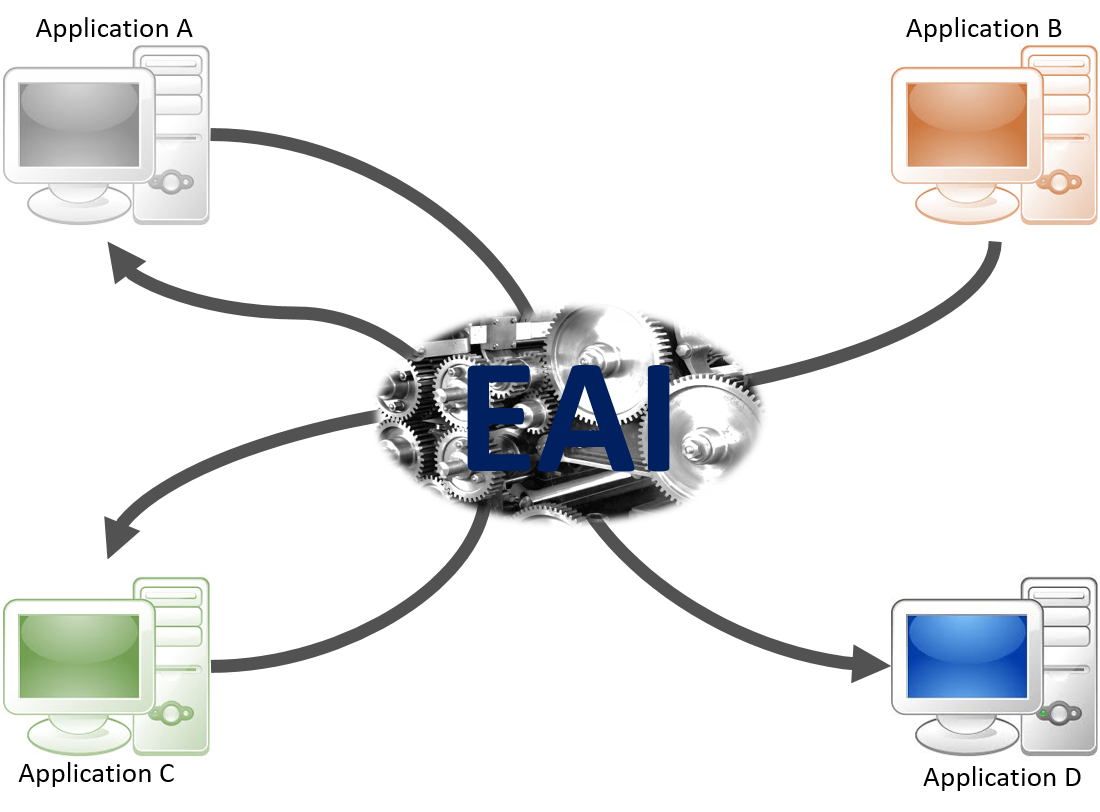
\includegraphics[width=10cm]{../img/eai_1.png}
				\caption{\label{Figure 1} L'EAI est un outil qui permet d'établir des
				routes entre applications métier.}
			\end{figure}
			
			Et les fonctions de l'EAI ne se résume pas au seul transport des données. Il
			est parfois utile de réaliser des actions sur les informations transmises
			d'une application à l'autre \ref{Figure 2}. Ces actions peuvent êtres par
			exemple :\newline
			\begin{itemize}
			  \item de valider les informations transmises. Par exemple, l'EAI va
			  s'assurer que pour chaque donnée émise par une application de gestion des
			  prescriptions, le nom du patient est bien présent.
			  \item d'effectuer des transformations. L'application destinataire ne
			  gère pas forcément les mêmes formats de données que l'application émettrice
			  car, rappelons-le, les applications ne sont pas forcément conçues pour
			  fonctionner ensemble. L'EAI est ainsi capable de faire des conversions de
			  format de donnée.
			\end{itemize}

			% Schéma détaillé EAI
			\begin{figure}
				\centering
				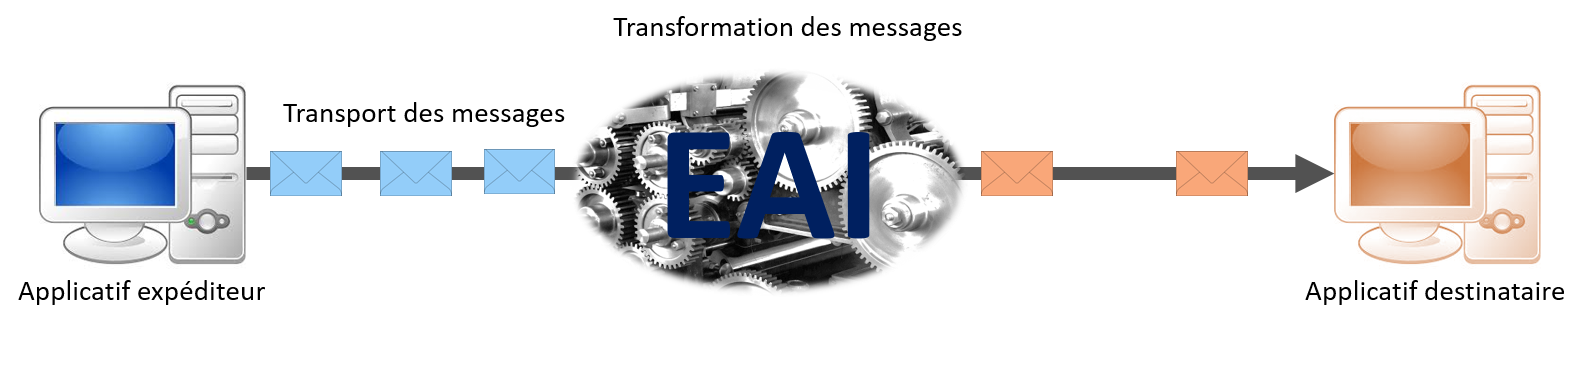
\includegraphics[width=15cm]{../img/eai_2.png}
				\caption{\label{Figure 2} Un EAI peut effectuer des opérations sur les
				données qui transite par lui.}
			\end{figure}
			
			\paragraph{}% Un peu de vocabulaire
 			Il existe un vocabulaire pour désigner les transferts de données entre
 			applications. Dans la suite, nous parlerons de :
 			\begin{description}
 				\item[Flux] Les flux sont tout simplement les routes permettant de
 				connecter une application à une autre. Dans un système d'information hospitalier
 				(SIH), il y a donc autant de flux de de couple d'application. Il est
 				possible - et même courent - qu'une application soit reliée à plusieurs
 				autres.
 				\item[Message] Les données qui passent le long des flux, d'une application
 				à une autre, sont appelés message. Les messages se présente en général sous
 				la forme de texte hautement standardisé. Les messages sont émis par les
 				applicatifs métier dans un format donné. Il existe de nombreux formats
 				dont certains sont spécifiques au monde hospitalier. L'annexe N présente
 				quelques-uns des principaux formats utilisés (HL7 et HPRIM).
 			\end{description}
%<<<<<< release1
		\subsubsection{Les flux de messages doivent être surveillés}
			\paragraph{}% Importance fonctionnelle de la supervision
			L'EAI est un outil complexe mais dont le bon fonctionnement est essentiel. En
			effet, c'est tout le SI de l'hôptial qui repose en permanance sur l'EAI. Si
			un disfonctionnement intervien au niveau de se dernier, des pans entier du
			service hospitalier risque d'en patir, ce qui aura des conséquences sur le
			traitement des patients.

			\paragraph{}% Exemple de cas de disfonctionnement
			Il existe différentes raisons pour lesquelles un flux peut tomber en erreur.
			La Figure 3 \ref{Figure 3} expose les trois principales. La cause (1) évoquée
			sur le schéma, correspond à une erreur qui survient entre l'application source et l'EAI,
			c'est-à-dire lors du transfert du message de l'application à l'EAI. Une
			erreur de ce type peut avoir des causes variées. Il peut s'agir d'un problème
			au niveau du réseau qui transporte les message (par exemple une coupure
			internet). Le cas (2) correspond à une erreur qui est levée
			lors du traitement du message par l'EAI. Il se peut que le contenu du
			message ne soit pas conforme à ce qu'attendait le script réalisant le
			traitement. Ce peut être par exemple le cas lorsqu'un utilisateur de
			logiciel métier fait un erreur de saisie et que cette erreur n'est pas
			relevée par le logiciel en question. Enfin, dans le cas (3), les messages
			s'accumulent à la sortie de l'EAI car la route entre l'EAI et l'application
			destinataire est bloquée, par exemple par une coupure momentanée du réseau.
			% Schéma des causes d'erreur
			\begin{figure}[!h]
				\centering
				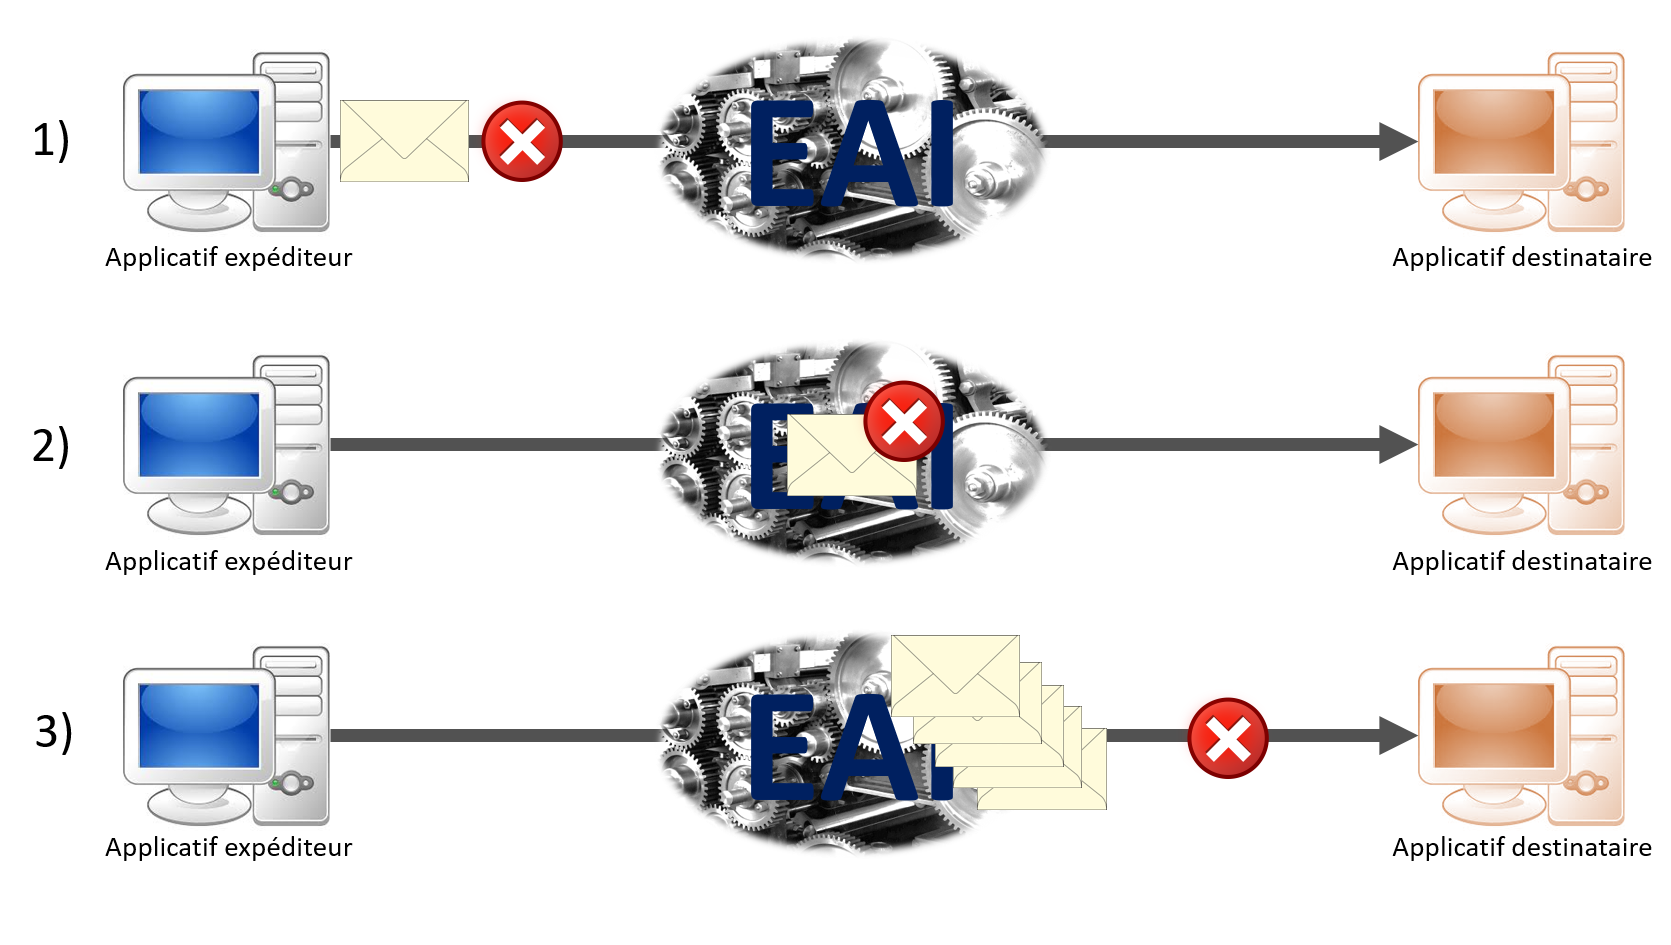
\includegraphics[width=15cm]{../img/error_1.png}
				\caption{\label{Figure 3} De multiples causes d'erreurs peuvent stoper
				momentanément un flux de message.}
			\end{figure}
			
			\paragraph{}% Surveiller un flux c'est pas facile
			Ainsi, il est capital d'exercer une surveillance continue sur les différents
			flux, pour être certain que l'EAI assure bien ses fonctions et que les
			messages transitent correctement. Cette surveillance est ce que l'on appel la
			supervision des flux. Cette tâche peut être assurée grâce à deux outils :
			\begin{itemize}
			  \item L'environnement de développement intégré (IDE) de Cloverleaf. Cet
			  outil permet de controler tout l'EAI, c'est-à-dire aussi bien assurer la
			  supervision que de mettre en place de nouveaux flux. L'IDE est un outil
			  très complexe qui nécéssite une formation spécialisée, ce que les
			  personnels des services informatiques des centres hospitaliers n'ont pas
			  forcément.
			  \item Les consoles de supervision.
			\end{itemize}
			
		\subsubsection{TrackCIS est un outil qui permet la supervision des flux}
			\paragraph{}% C'est quoi une console de supervision ?
			Une console de supervision permet d'assurer la surveillance
			de tout ou partie des flux gérés par l'EAI. Elle dispose d'un
			nombre limté de fonctionnalité par rapport à l'IDE mais se veut plus simple
			et plus rapide d'utilisation. Il esxiste actuellement pour Cloverleaf un
			certain nombre de consoles.
			
			\paragraph{}% Exemple de global monitor
			Il existe actuellement différentes consoles de supervisions dédiées à la
			surveillance des flux de Cloverleaf. En voici quelques exemples :
			\begin{description}
				\item[Global Monitor] Cette console est développée par le même éditeur qui
				est à l'origine de Cloverleaf : Infor. Global Monitor est un outil assez
				complexe, il est destiné à des personnes relativement rompuent au
				fonctionnement de l'EAI.
				\item[EAI Supervision] Cet outil est développé par l'un des plus gros
				éditeur de logiciels hospitalier français : Maincare. Cette console ne
				permet cependant pas de gérer tous les flux, mais selement ceux faisant
				intervenir des applications développées par Mainecare.
				\item[TrackCIS] Cette console à été développée par Xperis. Elle est destinée
				à des utilisateur ne maîtrisant pas forcément l'EAI.
			\end{description}
			
			\paragraph{}% Objectif de l'outil
			
			
			\paragraph{}% Les principales fonctionnalités
			
		
		\paragraph{}% Résumé de la partie 1.1
		Nous avons vu dans cette première partie que l'EAI est une solution au
		problème de l'onteropérabilité en établissant des flux de données entre
		applications métier. Nous avons souligné le fait que la surveillance (la
		supervision) continue des flux est indispensable au bon fonctionnement de
		l'EAI et, par extention, de tout le SI. Enfin, TrackCIS est un outil qui
		permet de rendre la supervision plus simple et plus rapide.\newline
		Dans la suite nous découvrirons les prblématiques inhérentes à cet outil.
		
	\subsection{TrackCIS est au cœur d'une problématique commerciale pour Xperis}
		\paragraph{}
		Précédement nous avons établi les bases des problématiques d'interopérabilité
		des établissements hospitalier. Xperis est une entreprise qui propose
		d'accompagner ces dernier dans la mise en place et le maintien d'un EAI :
		Cloverleaf.
		
		\subsubsection{Xperis est l'intermédiaire dans la distribution de Cloverleaf}
			\paragraph{}% Les acteurs de ce projet
			Les acteurs du projet qui nous concerne sont Xperis et les centres
			hospitaliers clients d'Xperis.
			\begin{itemize}
			  \item Xperis est le commanditaire du projet. Il est également un
			  utilisateur de TrackCIS.
			  \item Les centres hospitalier sont les utilisateurs finaux de la solution
			  que nous étudirons et implémenterons au cours de ce projet.
			\end{itemize}
			
			\paragraph{}% Présentation d'Xperis
			Le premier acteur de notre projet est la société Xperis. Cette entrepsrise
			Bordelaise est spécialisée dans le Consulting autour de l'EAI Cloverleaf.
			C'est une TPE (Très Petite Entreprise), qui compte une dizaine de personnes.
			6 consultants techniques, deux ingénieurs commerciaux, une responsable
			administrative et communication et un génrant
			
			\paragraph{}% Position d'Xperis sur le marché
			Xperis est le seul distributeur de CLoverleaf en France. L'entreprise fait le
			lien entre Infor et les éditeurs de logiciels hospitaliers. Les clients
			d'Xperis sont ces éditeurs.
			
		\subsubsection{Xperis cherche à établir des liens directs avec les hôpitaux}
			\paragraph{}% panorama du monde hospitalier
			Au 31 décembre 2014, on dénombrait en France 3 111 établissements hospitaliers, 
			dont 1 416 établissements publics. Ces derniers sont répartis en trois catégories 
			\citep{drees_panoramas_2016} :
			\begin{itemize}
				\item 182 centres hospitaliers régionaux (CHR) : ils dispensent des soins 
				spécialisés à la population de la région,
				\item 973 centres hospitaliers (CH) : ils assurent les soins médicaux, 
				chirurgie et prise en charge des personnes âgées,
				\item 97 centres hospitaliers psychiatriques,
				\item 164 établissements de soins longue durée.
			\end{itemize}
			Les hôpitaux privés sont répartis en deux catégories :
			\begin{itemize}
				\item 1 012 établissements privés à but lucratifs,
				\item 683 établissements à but non lucratifs, dont 21 centre de lutte contre 
				le cancer.
			\end{itemize}
			
			\paragraph{}% regroupement des hôpitaux en GHT
			Depuis 2016, une directive nationale prévoit le regroupement des établissements de 
			santé publics français en groupements hospitaliers de territoire (GHT) 
			\citep{valls_decret_2016}. Dans le cadre d'un GHT, les établissements doivent mettre 
			en commun leur système d'informations et doivent utiliser les mêmes logiciels et 
			applicatifs métiers. Le décret prévoit en outre la création de 135 GHT  
			\citep{touraine_marisol_2016}. Ceci risque d'impacter l'activité d'Xperis dans la 
			mesure où, lorsque les GHT seront vraiment formés, les outils d'interopérabilités 
			(les EAI) seront également mutualisés.
			
			\paragraph{}% Maincaire va peut-être se séparer d'Xperis un jour
			Le business-modèle d'Xperis repose donc sur les problèmes d'interopérabilité des 
			éditeurs. Or certains éditeurs cherchent à résoudre ce problème par eux-même. C'est 
			par exemple le cas de Maincare, le plus gros client d'Xperis. L'entreprise affiche 
			depuis quelques mois la volonté de développer sa propre solution d'interopérabilité 
			\citep{perochon_e-sante:_2016}. Le risque pour Xperis est donc, à terme, de perdre son 
			plus important client. Pour préparer cette éventualité, l'entreprise cherche de plus 
			en plus à traiter directement avec les établissements hospitaliers.
			
			\paragraph{}% La stratégie d'Xperis face à ces challenges
			
		\subsubsection{Un outil qui se vend mal et qui est peu utilisé}
			\paragraph{}% L'objectif initial du projet TrackCIS
			
			\paragraph{}% Les specs de départ de TrackCIS
			
			\paragraph{}% Le problème actuel avec cet outil
			
			% Résumé de la partie 1.2
			\paragraph{}
			Nous avons vu qu'Xperis est confronté à un certain nombre de problématiques
			commerciales. L'entreprise à une vrais volonté de traiter en direct avec les
			hôpitaux pour gagner en indpendance vis à vis des éditeurs. TrackCIS entre
			dans cette stratégie mais a du mal à se faire une place parmi les
			clients.\newline
			L'ensemble de ces problématiques constituent le socle du présent travail.
	
	\subsection{Vers une nouvelle version de TrackCIS}
		\paragraph{}% problème => solution commerciale ou solution fonctionnelle
		Le poblème que pose TrackCIS soulève une question : pourquoi cet outil ne se
		vend t-il pas ? La réponse à cette question, loin d'être triviale, pourrait
		être de deux type : une solution commerciale et une solution fonctionnelle.
		\begin{description}
			\item[La solution commerciale] Nous faisons ici l'hypothèse que la cause au
			fait que TrackCIS ne se vende pas est commerciale. Ceci pouvant impliquer
			plusieurs chose comme le fait que :
			\begin{itemize}
			  \item les clients n'ont pas réellement besoins d'un outil tel que TrackCIS.
			  Il esxiste en effet d'autres outils de supervision pour Cloverleaf, comme
			  par exemple l'outil Global Monitore, dont nous reparlerons un peu plus
			  loin, ou encore EAI Supervision.
			  \item les utilisateur de TrackCIS n'existent pas. Cet outil a été développé
			  pour des personnes non initiées à Cloverleaf mais qui pour qui il serait
			  intéressant de superviser quelques flux.
			  Or il est tout à fait possible que ce type de personne n'existe pas ou pas
			  encore dans les hôpitaux.
			  \item la communication ou le démarchage autour de TrackCIS est insufisant
			  ou non adapté.
			\end{itemize}
			\item[La solution fonctionnelle] Cette fois-ci notre hypothèse est que
			TrackCIS ne se vend pas car il lui manque des fonctionnalité indispensables à
			ses utilisateurs.
		\end{description}
		
		\subsubsection{Comprendre les utilisateurs et leurs besoins}
			\paragraph{}% Nous ne traitons que de la solution fonctionnelle
			De ces deux solutions à la problématique soulevée par TrackCIS (commerciale
			ou fonctionnelle), nous prenons le partie de n'en traiter qu'une, la
			seconde.\newline
			L'objectif assumé de ce mémoire est de traiter de l'amélioration
			fonctionnelle et technique d'un outil tel que TrackCIS. Notre objectif est de
			chercher à connaitre
			
			\paragraph{}% Les anciennes specs ne permettent pas de bien comprendre le besoin des utilisaturs
			
			\paragraph{}% Ce qui soulève la question de qui sont les utilisateurs
			
		\subsubsection{Un module statistique lié aux évolutions de Cloverleaf}
			\paragraph{}% Volonté de développer un module stat
			Une volonté liée à l'implémentation de cette fonctionnalité dans Cloverleaf depuis 
			la nouvelle version. De plus, les statistiques sont actuellement assez mal 
			exploitées par les autres outils.
			
			\paragraph{}% Les atous d'un tel module
			Avantage concurentiel, vision globale sur l'état des flux, du SI\ldots
			
		\subsubsection{Méthodologie générale du projet}
			\paragraph{}% Résumé des problèms soulevés
			Nous avons constaté dans les parties précédentes plusieurs problématiques
			inhérentes à TrackCIS. Nous avons également pris le partie de tenter de
			répondre à ces problèmatiques selon une logique fonctionnelle, de qui
			implique de développer de nouvelles fonctionnalités sur cet outil.
			
			
			\paragraph{}% Cadrage de notre travail
			Avant d'exposer la méthodologie suivie dans ce projet, fixons les limites de
			ce projet. Nous ne nous intéresserons ici qu'au développement d'un
			module d'affichage de statistiques dans TrackCIS. Les raisons à ce choix sont
			:
			\begin{itemize}
			  \item Le développement d'un tel module est un objectif prioritaire pour
			  Xperis concernant TrackCIS.
			  \item La possibilité de récupérer des statistiques sur le fonctionnement de
			  Cloverleaf est une fonctionnalité nouvelle de l'EAI. Aucune console de
			  supervision n'en n'a pour l'instant totalement exploité les possibilité.
			  \item De ce fait, ce nouveau module peut apporter un facteur de
			  différentiation notable à TrackCIS par rapport aux outres consoles.
			  \item Ceci pourrait apporter une solution à la problématique commerciale
			  de TrackCIS, à savoir le fait qu'il s'en vend peu.
			\end{itemize}
			Cependant, l'implémentation de ce seul modul statsitque n'apporterait une
			réponse fonctionnelle complète. En effet, les besoins des utilisateurs sont à
			ce jour mal connus par l'entreprise. La typologie même de ces utilisateur est
			aujourd'hui difficile à définir.\newline
			Notre objectif est donc le suivant :\newline
			Contribuer à l'amélioration de TrackCIS par l'implémentation d'un module de
			statstiques et par une analyse des besoins dans le but de propositions
			d'autres axes d'amélioration.

			\paragraph{}% Méthodologie générale + présentation de l'approche
			% fonctions -> comportements -> structure de Xavier Blanc
			Pour ce faire, nous procéderons en trois grandes étapes : l'analyse du
			besoin, la conception d'une solution et le développement de cette
			solution. Au cours de chacune de ces étapes nous serons amener  modéliser
			différents aspect de l'application, notament 3 :
			\begin{itemize}
			  \item Modélisation des fonctions de l'application
			  \item Modélisation des comportement de l'application et des utilisateurs
			  \item Modélisation de la structure de l'application
			\end{itemize}
			Nous nous bason ici sur le
			
			Dans le livre intitulé UML2, Xavier Blanc et Isabelle mounier présente une
			méthodologie d'analyse et de conception en trois étapes.
			
			\paragraph{}% Détail pour la phase d'analyse du besoin
			
			
			
			